\begin{question}[name=Spørsmål, topic=tyristor]
	Tegn symbolene for følgende komponenter.
	\begin{enumerate}[label=\roman*]
		\item Halvlederdiode
		\item LED
		\item Zenerdiode
	\end{enumerate}
\end{question}


\begin{solution}[name=Løsningsforslag]
tatata

%	\begin{figure}[H]
%		\centering
%		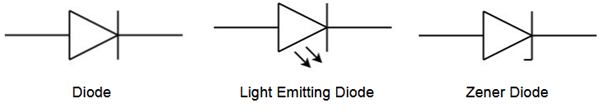
\includegraphics[width=0.7\textwidth]{diode/figurer/oppgave1.png}
%		\caption{Eksempel på forskjellige diode symboler.}
%		\label{fig:diodeSeeeymb}
%	\end{figure}
\end{solution}